\documentclass[conference,a4paper]{IEEEtran}
\bibliographystyle{IEEEtran}

\usepackage[utf8]{inputenc}
\usepackage[T1]{fontenc}
\usepackage[frenchb]{babel}
\usepackage{flushend} % Equalizes columns on last page
\usepackage{graphicx}

\title{%
  Implémentation d'un outil
  de reconstruction de graphes de flot de contrôle
  pour l'analyse temporelle
  par vérification de modèles}

\author{%
  \IEEEauthorblockN{Armel Mangean}
  \IEEEauthorblockA{%
    Institut de Recherche en Communications et Cybernétique de Nantes\\
    %IRCCyN UMR CNRS 6597 \\
    École Centrale de Nantes, LUNAM Université \\
    Nantes, France}}

%% TODO
%% simplification

\begin{document}
  \maketitle

  \begin{abstract}
  L'analyse temporelle des systèmes embarqués temps-réel est nécessaire pour
  garantir le respect de l'ensemble de leurs contraintes temporelles. Une telle
  analyse doit déterminer si l'ensemble des exécutions possibles d'un système
  respecte l'ensemble des ses contraintes temporelles. Les différentes analyses
  temporelles existantes s'appuient sur un modèle du programme et un modèle de
  la plateforme matérielle.
  
  Cet article décrit l'implémentation d'un outil de génération de modèles de
  programmes pour l'analyse temporelle par vérification de modèles
  temporisés. Le processus de génération est composé de deux étapes. La première
  réalise une reconstruction du graphe de flot de contrôle du programme à partir
  d'un fichier éxécutable. La seconde procède à une \textit{simplification} du
  graphe de flot de contrôle par \textit{slicing}.
\end{abstract}

  %% * Résumé *

  \renewcommand{\baselinestretch}{1.2}
\section{Introduction}
\label{sec:introduction}

  % Nécessité de l'analyse temporelle pour le temps-reél.
  L'analyse temporelle d'un systèmes temps réel doit déterminer si l'ensemble
  des exécutions possibles de ce système respecte les  contraintes temporelles
  exprimées dans sa spécification.  Pour réaliser cette analyse, il faut
  connaître les pires temps d'exécution des tâches qui composent le logiciel du
  système. Ces valeurs sont généralement impossibles à calculer mais il est en
  revanche possible d'en calculer des bornes supérieures.
  Parmi les différentes techniques développées pour cela, nous
  nous intéressons à celles basées sur la théorie de la vérification des
  systèmes temporisés~\cite{DOT10, CB13}. La borne y est
  déterminée en cherchant le plus long chemin dans un modèle obtenu par
  composition d'un modèle du code binaire de la tâche et d'un ensemble de
  modèles des composants de l'architecture matérielle (processeur, pipeline,
  mémoires caches, bus, etc.). Comparées aux autres approches, ces
  techniques permettent une modélisation moins abstraite des comportements
  matériels, ce qui permet d'obtenir des bornes plus
  précises. En revanche, leur application reste limitée par l'explosion
  de la taille l'espace d'état du modèle à analyser~\cite{Wil04}.

  Dans la continuité de~\cite{CB13}, nos travaux visent à
  contribuer au contrôle de la taille de l'espace d'état en réalisant une
  abstraction du code binaire. Cette abstraction consiste à limiter
  l'état du modèle aux valeurs des registres et mots mémoire qui ont un
  impact sur le flot de contrôle. Le calcul de cette abstraction se fait en
  deux étapes. D'abord, le graphe de flots de contrôle du programme est
  reconstruit. Ensuite, ce graphe est analysé \emph{via} un \emph{program slicing}
  pour calculer le sous-ensemble des registres et mots mémoires pertinents.
  Dans la suite, nous nous concentrons sur cette seconde étape.

  %Notre outil est implémenté en C++ et utilise la bibliothèque de manipulation
  %de graphe LEMON \cite{DJK11}.  Les sections \ref{sec:reconstruction} et
  %\ref{sec:slicing} détaillent les aspects théoriques de notre outil. La
  %section \ref{sec:implementation} détaille l'implémentation de notre outil.
  %Enfin, la section \ref{sec:conclusion} présente les perspectives de ce
  %travail.



  %% * Introduction *
  %% ~ Pourquoi l'"analyse temporelle"
  %%   > une nécessité pour le temps-réel (pourquoi)
  %% ~ Pourquoi la "reconstruction de CFG"
  %%   > une nécessité pour l'analyse temporelle (pourquoi)
  %% ~ Pourquoi la "vérification de modèles"
  %%   > interet de la vérification de modèles (pourquoi)
  %%   > figure explicite de l'analyse temporelle par vérification de modèles
  %% ~ Organisation de l'article

  \section{Reconstruction de CFG}
\label{sec:reconstruction}

  % Limitation des approches de reconstruction de CFG à partir des fichiers
  % sources et nécessité du fichier exécutable pour la reconstruction de CFG.

  Les instructions machine, ou simplement instructions, sont les opérations de
  base codées en langage machine que peut manipuler un processeur. Un fichier
  exécutable contient l'ensemble des instructions d'un programme. Ce type de
  fichier est généralement produit par la compilation des fichiers sources d'un
  programme écrits dans un langage de haut niveau -- un langage de programmation
  -- vers un langage de bas niveau -- le langage machine.

  Certaines méthodes de reconstruction de CFG s'appuient sur les fichiers
  sources des tâches. Cependant, le comportement logiciel qui est effectivement
  constaté à l’exécution n’est pas strictement celui que définissent les
  fichiers sources en langage de haut niveau mais celui que défini le fichier
  exécutable associé en langage de bas niveau. Or, il existe par nature une
  différence d’expressivité entre les langages de haut et de bas-niveau. De
  fait, le processus de compilation équivaut le plus souvent à une fonction de
  traduction non-injective des premiers vers les seconds. De plus, il est très
  fréquent que le processus de compilation inclut une phase d'optimisation du
  fichier exécutable. Les instructions machine y sont modifiées, fusionnées,
  dupliquées, ou réordonnées. L'élément essentiel à une reconstruction précise
  d'un CFG, et a fortiori d'une analyse temporelle précise, est donc le fichier
  exécutable issu de la compilation des fichiers sources du programme considéré.

  \vspace{1em}

  % Définition de CFG et bloc de base

  Un bloc de base est une séquence d'instructions qui n'a qu'un point d'entrée,
  sa première instruction, et qu'un point de sortie, sa dernière instruction.
  Le graphe de flot de contrôle d'un programme est un graphe orienté dans lequel
  les noeuds représentent les blocs de base issus du programme et les
  transitions représentent les enchainements possibles entre les différents
  blocs de base lors de l'exécution du programme. De manière formelle, un CFG
  est un tuple $G = (V, E, u, v)$, où les noeuds $V$ correspondent aux blocs de
  bases, les transitions $E \subset V \times V$ sont les chemins du flot de
  contrôle, $u \in V$ représente le n{\oe}ud d'entrée et $v \in V$ le n{\oe}ud
  de sortie.

  % Principes de recontruction des blocs de base
  
  \begin{figure}[ht]
    \centering
    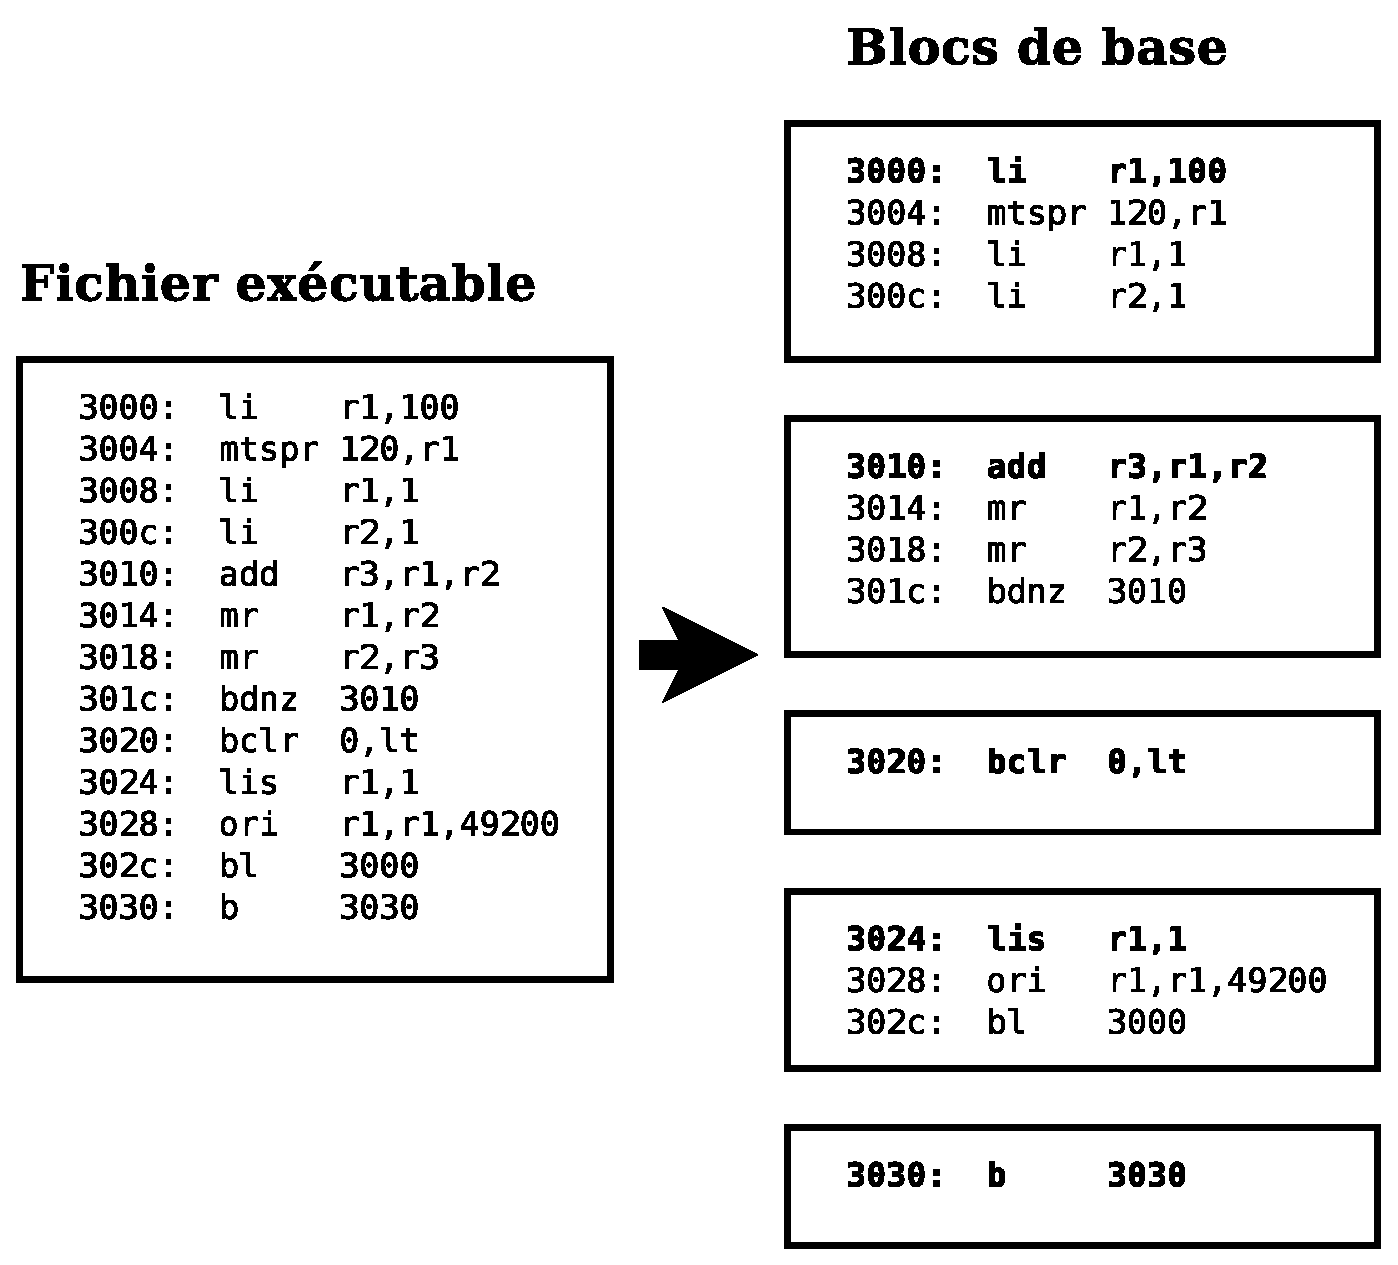
\includegraphics[scale=0.3]{img/recons1.eps}
    \caption{Processus de reconstruction de blocs de base}
    \label{fig:recons1}
  \end{figure}

  Afin de procéder à la reconstruction du CFG d'une tâche, il est tout d'abord
  nécessaire d'en reconstruire les blocs de base. Pour cela il faut identifier
  les points d'entrée de ses différents blocs de base. Une instruction est une
  entrée de bloc de base si elle se trouve être :
    \begin{itemize}
      \item le point d'entrée du programme ;
      \item une cible de saut ;
      \item immédiatement après une instruction de saut ;
      \item la première instruction du fichier exécutable.
    \end{itemize}
  Les blocs de base sont ensuite construits séquentiellement par accumulation
  des instructions se trouvant entre un point d'entrée de bloc de base inclus
  jusqu'au point d'entrée suivant exclus. La figure \ref{fig:recons1} donne un
  exemple d'un telle reconstruction.

  % Utilisation d'un analyseur sémantique de fichiers exécutables pour la
  % reconstruction de CFG.

  Les informations nécessaires à la classification des instructions utiles à la
  reconstruction des blocs de base sont issues d'une analyse syntaxique et
  sémantique du fichier exécutable produite par l'outil \textsc{HARMLESS}
  \cite{KBB12}.
  
  % Principes de recontruction des CFG

  \begin{figure}[ht]
    \centering
    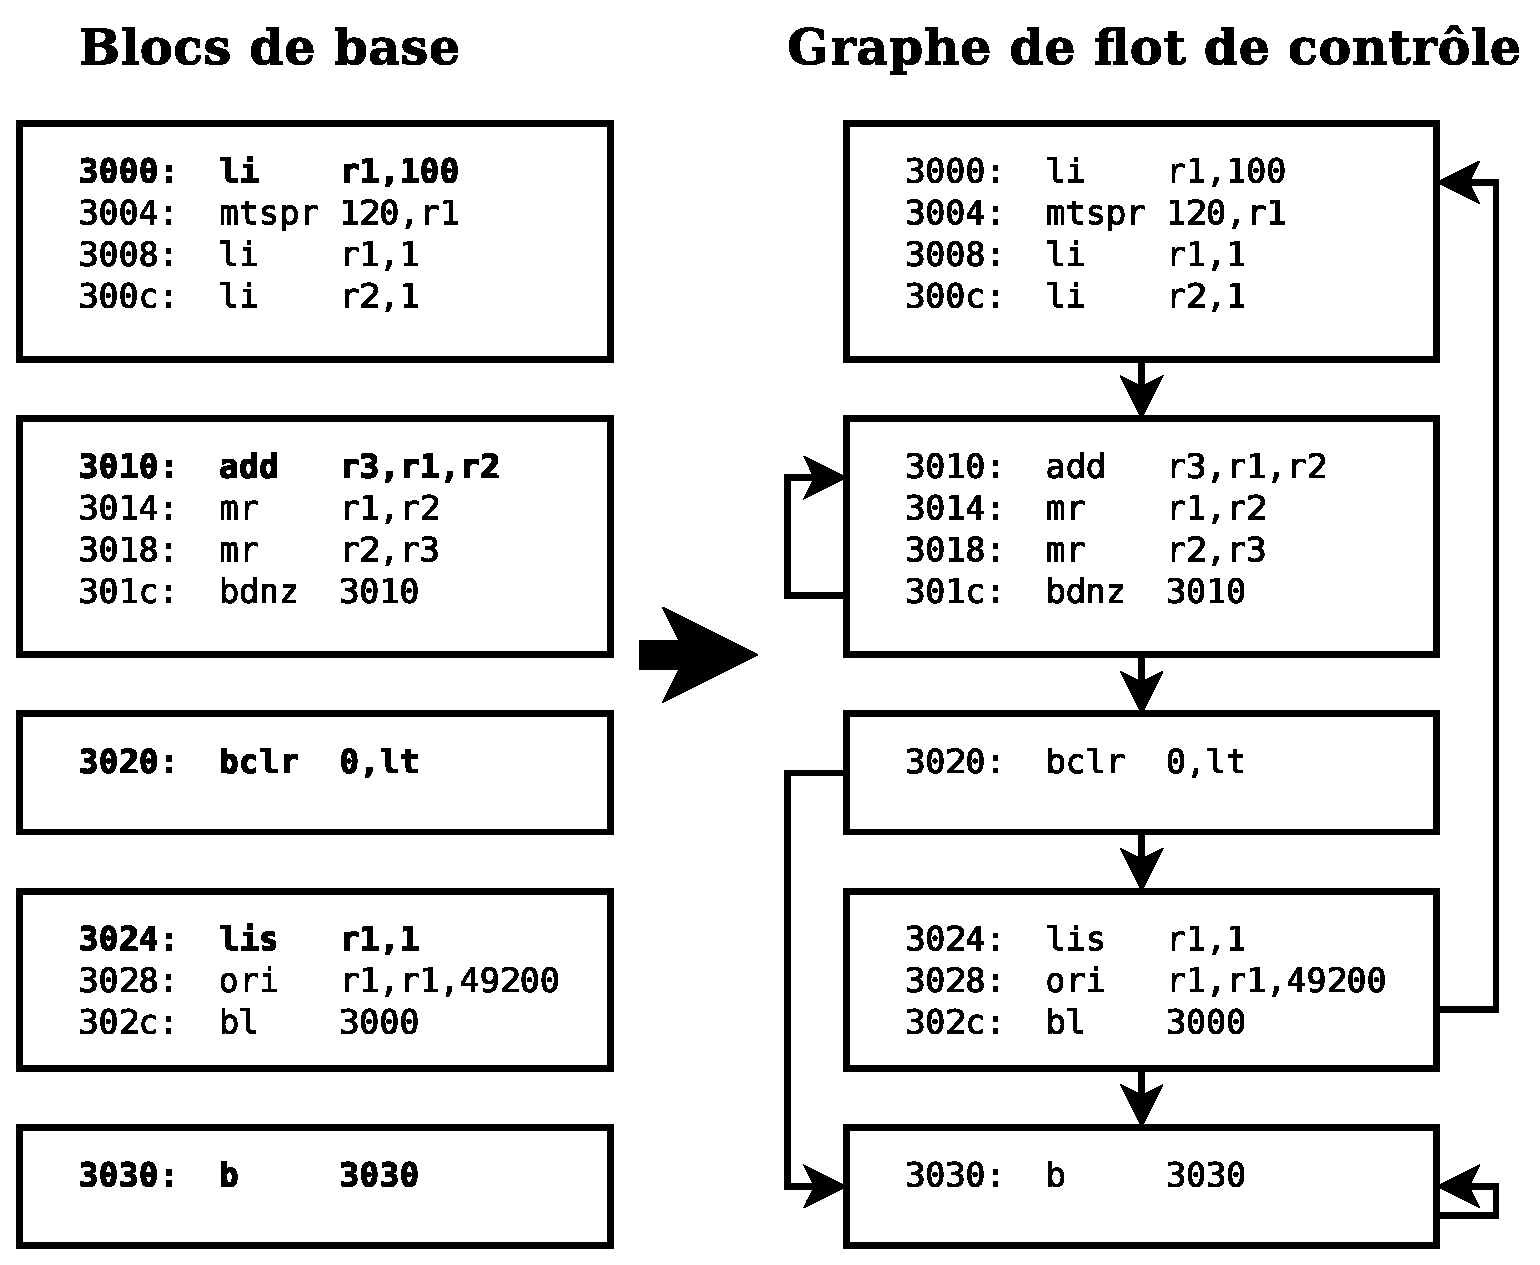
\includegraphics[scale=0.3]{img/recons2.eps}
    \caption{Processus de reconstruction d'un CFG}
    \label{fig:recons2}
  \end{figure}
    
  Pour reconstruire un CFG il est tout d'abord nécessaire d'identifier les
  noeuds. C'est une tâche triviale vis-à-vis de la définition d'un CFG. Il faut
  également identifier le n{\oe}ud d'entrée. C'est le n{\oe}ud correspondant au
  bloc de base issu du point d'entrée du programme. Il faut ensuite en retrouver
  les transitions. Elles sont obtenues itérativement en associant à chaque bloc
  de base les cibles possibles de son point de sortie. La figure
  \ref{fig:recons2} donne un exemple d'un telle reconstruction. Lorsqu'il n'est
  pas trivial de déterminer la cible d'un saut, comme cela peut l'être dans le
  cas de sauts indirects. il est fait usage à ce moment de la reconstruction
  d'un noeud inconnu. Les cibles des ces sauts sont déterminées par la suite.

  %% Utilisation de la propagation de constante pour rafiner le CFG.

  Afin de permettre la déterminaison de certaines cibles de saut il est une
  nouvelle fois fait usage de l'outil \textsc{HARMLESS}. Celui-ci réalise une
  simulation de l'exécution de notre programme sur la plateforme matérielle
  considérée. Il est donc possible de procéder à une propagation de constantes
  permettant de déterminer des plages de valeurs pour certains registres.

  %% * Reconstruction *
  %% ~ Comment la "reconstruction de CFG"
  %%   > à partir de fichiers exécutables (pourquoi)
  %%   > à base de graphes (comment + définir "use-definition")
  %%   > par analyse sémantique des instructions (comment)

  \section{\textit{Simplification} de CFG}
\label{sec:simplification}

  % Program Slicing

  Le \textit{program slicing}, ou \textit{slicing}, est le calcul d'un
  ensemble d'instructions d'un programme qui affecte les valeurs des
  variables à un certain moment de l'exécution de celui-ci. Un
  \textit{slice} est donc un sous-ensemble d'instructions apartenant à
  l'ensemble des instructions du programme. Ce sous-ensemble
  d'instructions est tel qu'il possède un comportement équivalent au
  programme originial vis-à-vis de la valuation d'un sous-ensemble de
  variables du programme.

  Quand le \textit{slicing} s'applique à une seule procédure monolithique on
  parle de \textit{slicing} intraprocédural. En revanche lorsque le
  \textit{slicing} s'applique à un programme entier, au delà des frontières
  d'une procédure, on parle de \textit{slicing} interprocedural.

  \vspace{1em}

  % Intérêt du Program Slicing des CFG pour la vérification de modèle.

  Pour pallier au problème de l'explosion de l'espace d'état inhérent à la
  vérification des modèles il est nécessaire de réduire au maximum la quantité
  d'informations qui définit l'état du système. Le \textit{slicing} des CFG permet
  de ne conserver dans l'espace d'état du système uniquement les informations
  définissant l'état des variables -- registre ou contenu de la pile -- dont la
  valuation influt directement sur le flot de contrôle.

  Il n'est, en effet, pas nécessaire de conserver dans l'espace d'état du
  système les valuations de toutes les variables qui n'agissent pas directement
  sur le flot de contrôle puisqu'elles n'influent pas sur le temps d'exécution.
  
  \vspace{1em}
  
  % Program Slicing à base de graphes

  \begin{figure}[ht]
    \centering
    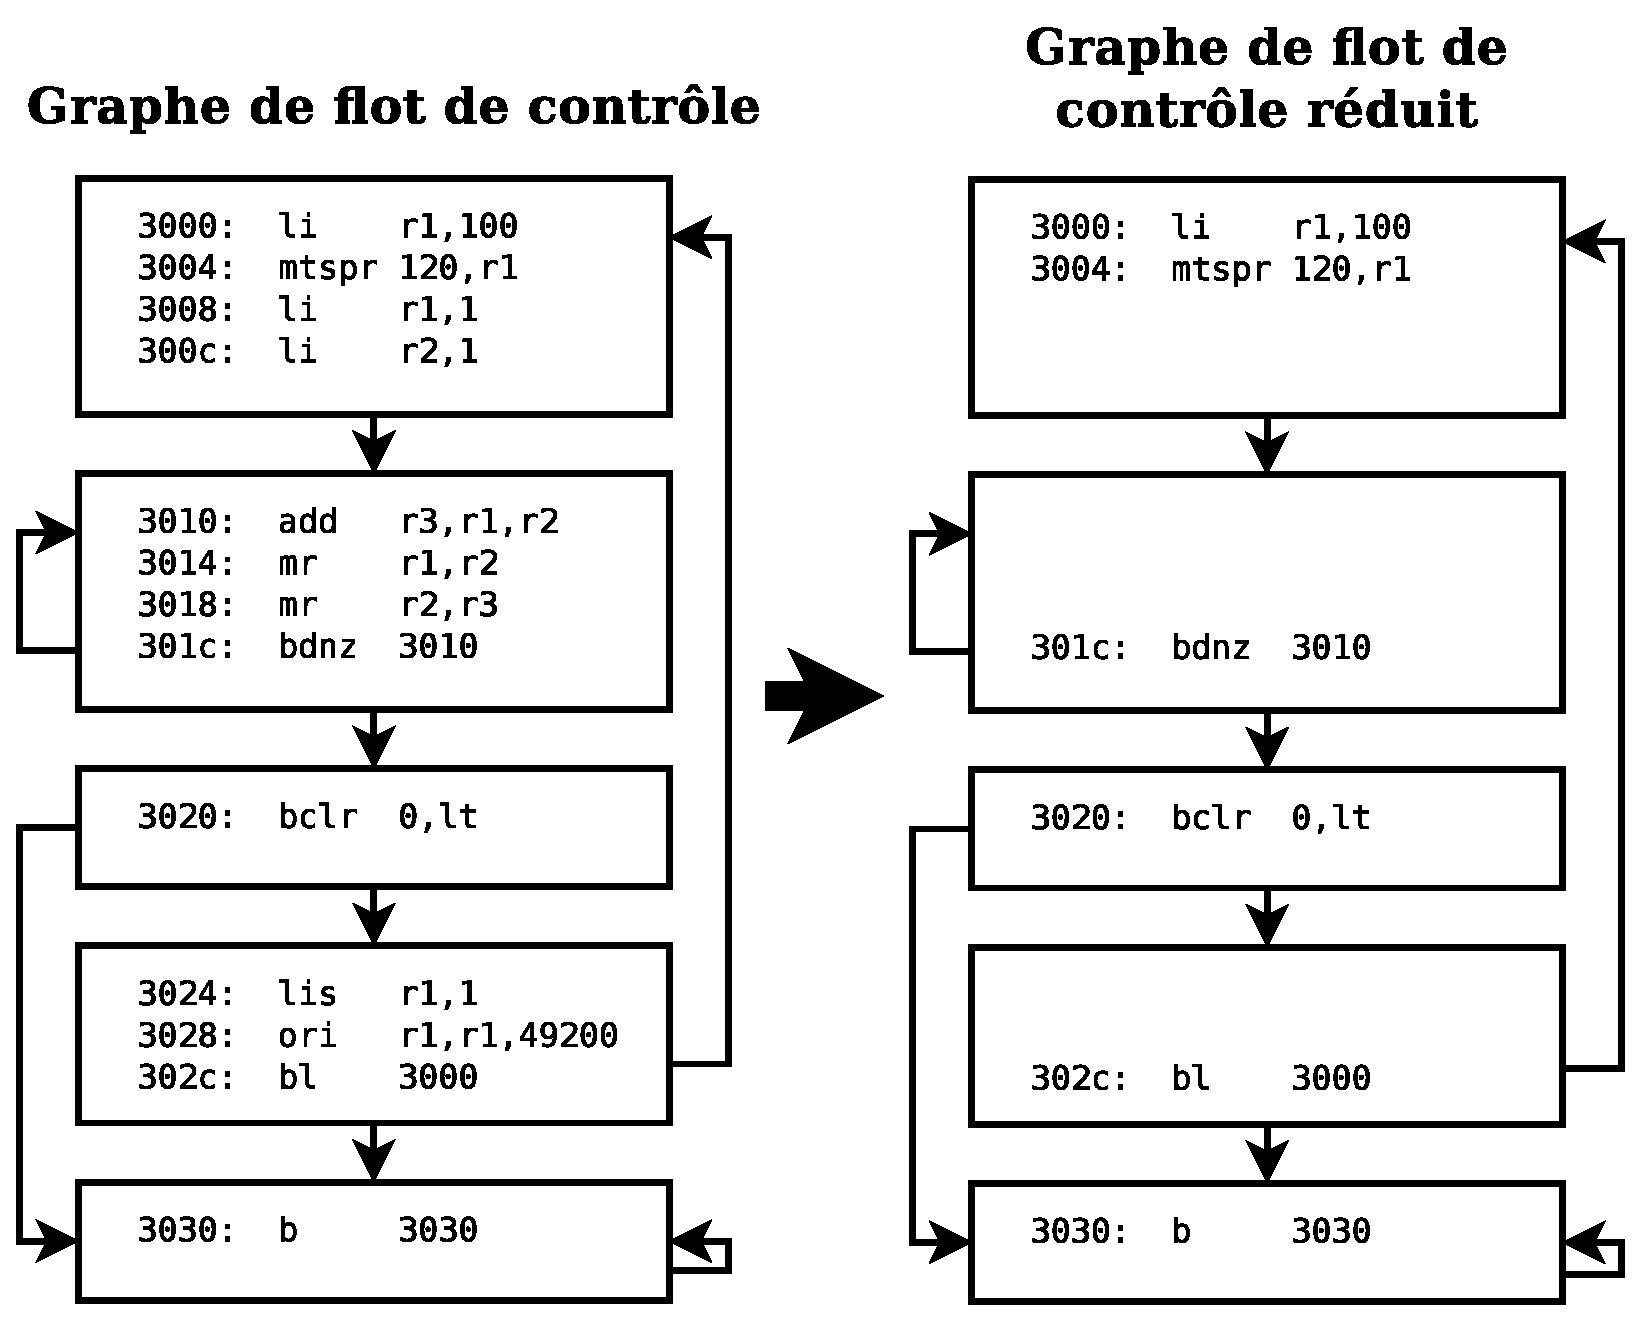
\includegraphics[scale=0.3]{img/slicing.eps}
    \caption{Processus de \textit{slicing} d'un CFG}
    \label{fig:slicing}
  \end{figure}
    
  Soit le CFG $G = (V, E, u, v)$. Un n{\oe}ud $d \in V$ domine
  (resp. post-domine) un n{\oe}ud $n \in V$ si et seulement si tous les chemins
  reliant $u$ (resp. $v$) et $n$ passent par $d$. Par définition, chaque
  n{\oe}ud se domine et post-domine lui-même. Un n{\oe}ud $d$ domine
  (resp. post-domine) strictement un n{\oe}ud $n$ si $d$ domine
  (resp. post-domine) $n$ et si $d$ n'est pas le n{\oe}ud $n$.

  Le dominateur (resp. post-dominateur) immédiat d'un n{\oe}ud $n$ est le
  n{\oe}ud qui domine (resp. post-domine) strictement $n$ mais qui ne domine
  (resp. post-domine) strictement aucun autre n{\oe}ud qui domine
  (resp. post-domine) strictement $n$. Tous les n{\oe}uds de $V$ ont un unique
  dominateur (resp. post-dominateur) immédiat excépté $u$ qui n'en a pas. Un
  arbre dominateur (resp. post-dominateur) est un graphe où l'ensemble des
  voisins d'un n{\oe}ud constitue l'ensemble des n{\oe}uds qu'il domine
  (resp. post-domine) immédiatement. Comme le dominateur (resp. post-dominateur)
  immédiat est unique, ce graphe est un arbre. Le n{\oe}ud d'entrée du CFG $u$
  est la racine de l'arbre.

  \vspace{1em}
  
  L'algorithme de \textit{slicing} implémenté s'appuie sur la méthode
  évoquée ci-après -- cf. \cite{CF97}. Les dépendances de données du
  programme y sont représentées par l'arbre post-dominateur et par des
  chaines de \textit{use-definition}. Ces chaines relient chaque
  utilisation d'une variable aux définitions qui peuvent l'affecter.

  Les dépendances de contrôle du programme sont manipulés à travers un graphe de
  dépendance de contrôle. Un graphe de dépendance de contrôle est un graphe où
  les arcs signifient un lien de dépendance entre la valuation du n{\oe}ud origine
  et l'exécution du n{\oe}ud cible.

  %% * simplification *
  %% ~ Comment la "simplification de CFG"
  %%   > par program slicing (comment et pourquoi)

  \section{Travaux connexes}
\label{sec:related-work}

  % Limitation de la de reconstruction de CFG compiler-aware et
  % annotation-based.

  Certaine méthodes de reconstruction de CFG s'appuient sur une connaissance des
  mécanismes internes des compilateurs. D'une part, cette connaissance n'est
  permise que par un travail fastidieux d'analyse des compilateurs. D'autre
  part, les mécanismes internes des compilateurs ne sont pas toujours librement
  accessibles. D'autres méthodes produisent des CFG imprécis qui doivent être
  annotés par la suite, notamment le nombre d'itérations maximal par boucle. De
  la même façon, ces méthodes dépendent d'un travail fastidieux, non sûr et non
  précis d'annotations.

  % FLP15: "Insight: An Open Binary Analysis Framework".

  L'outil \textsc{INSIGHT}, par exemple, n'est pas sujet à ces limitations
  \cite{FLP15}. Dans un permier temps le binaire est transposé dans une
  représentation intermédiaire sur laquelle est réalisée une analyse
  statique. Cette analyse est réalisée par une exécution symbolique de la
  représentation abstraite dans un domaine abstrait où chaque variable est
  substituée par une formule représentant toutes les valeurs possibles que
  celle-ci peut prendre. Pour ce faire, cet outil se base sur un solveur SMT.

  % The00: "Extracting Safe and Precise Control Flow from Binaries".

  Une autre approche, ascendante, classifie chaque instruction complètement et
  correctement avant de réaliser une analyse. Cette approche définit un CFG
  interprocédural (ICFG) en tant que la conjonction d'un graphe d'appel (CG) et
  de CFG, un par fonction. L'ICFG approximé est construit en deux étapes : un
  ICFG conservatif est construit, une analyse statique à base de propagation de
  constantes est réalisée pour raffiner l'ICFG précédent \cite{The00}.

  % Une approche similaire
  % CB13: "Timing Analysis of Binary Programs with UPPAAL".

  Enfin, une dernière méthode \cite{CB13} permet la génération d'un modèle
  logiciel basé sur la reconstruction automatique de CFG à partir de l'analyse
  exclusive d'un fichier binaire, cette génération est effectuée en deux
  phases. Durant la première le graphe de flot de contrôle de l'exécutable est
  reconstruit par \textit{program slicing} \cite{Wei81, Tip95}. Durant la
  seconde étape il est réduit, afin de contenir l'explosion de l'espace d'état,
  également par \textit{program slicing}. L'implémentation décrite ici s'appuie
  sur cette méthode.

  \vspace{1em}

  % Program Slicing à base d'arithmétique
  % Wei81: "Program Slicing".

  Dans sa définition originale l'algorithme de \textit{program slicing} fait
  usage d'un critère de \textit{slicing} et d'un ensemble d'équations pour
  déterminer quelles instructions font partie d'un \textit{slice} \cite{Wei81}.
  Une autre définition utilise une extension du concept de graphe de dépendence
  du programme pour créer des \textit{slices} intraprocéduraux précis pour
  les programmes structurés formés d'une seule procédure et développe le concept
  de graphe de dépendence du système (SDG) pour produire des \textit{slices}
  interprocéduraux précis tenant compte du contexte d'appel de chaque procédure
  \cite{HRB90}.

  Des techniques similaires ont été inventées pour fonctionner avec des
  programmes ayant des flots de contrôle arbitraires. Pour ce faire le CDG est
  construit à partir d'un CFG augmenté et le graphe de dépendance de données
  correspondant à partir du CFG original \cite{BH93, CF94}.

  Une méthode équivalente mais qui ne modifie pas le CFG ou le SDG a été
  développée \cite{Agr94}. Elle s'appuie sur un arbre des postdominants, créé en
  parallèle de la construction du SDG, ainsi qu'un arbre des successeurs
  lexicaux pour déterminer quel saut ajouter au \textit{slice} final.
  
  %% % KJL03: Interprocedural static slicing of binary executables

  %% Une autre méthode défini un procédé pour construire un CFG interprocédural
  %% \cite{KJL03}. Les algorithmes de construction des CFG, CDG, DDG et PDG y sont
  %% modifiés ou étendus pour tenir compte des spécificités des fichiers
  %% exécutables. Des analyses de dépendance de contrôle et de dépendance données
  %% sont réalisées pour chaque fonction du CFG. Un CDG et un DDG sont construits
  %% suite à ces analyses ainsi qu'un PDG grâce aux CDGs et DDGs. Des
  %% \textit{slices} intraproceduraux peuvent être calculés en utilisant le PDG
  %% ainsi que des \textit{slices} interproceduraux en incorporant le PDG au
  %% SDG.
  
  \vspace{1em}

  % Limitation des approches basées sur l'Abstract Interpretation et l'Integer
  % Linear Programming pour l'analyse temporielle.

  Quant à l'analyse temporelle en elle-même, différentes approches
  existent. Certaines se basent par exemple sur la prédiction des comportements
  matériels par interprétation abstraite et sur l'enumération implicite des
  chemins par optimisation linéaire en nombres entiers \cite{HF04}. Cependant,
  ces techniques définissent des algorithmes \textit{ad hoc} pour tenir compte
  des spécificités des architectures pour lesquelles l'analyse temporelle se
  porte. Un changement d'architecture implique alors l'écriture d'un nouvel
  algorithme. De plus les résultats actuellement obtenus avec ces méthodes
  surestiment significativement les bornes supérieures des temps d'exécutions
  réel. Cela peut s'expliquer par le fait que les modèles des comportements des
  équipements matériels qui y sont manipulés sont très abstraits.

  %% * Travaux connexes *
  %% ~ Alternative à notre "reconstruction de CFG"
  %%   > limitations des autres approches
  %%   > slicing à base d'arithmétique
  %%   > approche similaire (comparaison à CB13)

  \section{Conclusion}
\label{sec:conclusion}

  % Résumé.

  Cet article décrit le fonctionnement d'un outil de génération de modèles de
  programmes pour l'analyse temporelle des systèmes embarqués temps-réel par
  vérification de modèles temporisés. Les modèles produits sous forme
  d'automates finis sont générés à partir de fichiers exécutables suivant une
  approche de reconstruction de CFG à base de graphes. Ces modèles sont délestés
  d'un certain nombre d'informations qui ne sont pas nécessaires à l'analyse
  temporelle afin de contenir la taille de l'espace d'état qu'ils engendrent.

  % Perspectives associées.

  Les microprocesseurs multi-c{\oe}urs sont de plus en plus employés dans
  l'embarqué temps-réel à des fins de performances et de baisse de consommation
  d'énergie. La réalisation de cet outil fait partie d'un travail de
  développement d'une approche d'analyse temporelle adaptée à ces plateformes
  matérielles.


  %% * Conclusion *
  %% > Ajouter les perspectives

  \bibliography{refs.bib}
\end{document}
